\section{Practical Middleware for Massively Multiplayer Online Games}
The first architecture and it's design choices we are going to review, is the architecture described in \emph{Practical Middleware for Massively Multiplayer Online Games} \cite{middleware}.
In this paper the authors elaborated on the middleware platform. The purpose of such a platform  is, how the authors stated it, "Middleware helps programmers manage the complexity and heterogeneity of distributed computing environments". So for short it is a platform which makes it easier to develop and maintain distributed games. The authors have also developed their own platform and have made several architectural design decisions for that. The platform is called Distributed organized Information Terra (DoIT) middleware platform. \\

\begin{wrapfigure}{r}{0.5\textwidth}
\begin{center}
  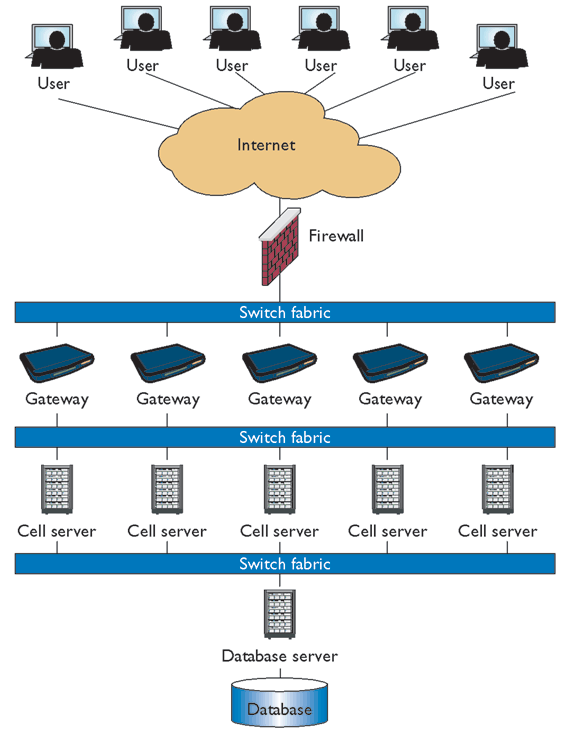
\includegraphics[width=0.4\textwidth]{4tier}
  \label{fig:4tier}
  \caption{General framework for middleware platforms for MMOG}
\end{center}
\end{wrapfigure}

\noindent A lot of research has been done by researchers to defina a framework for middleware platforms. The framework is a 4-tier architecture consisting of a client, a proxy/gateway, a cell server and a database tier. The gamers have control over the client applications. The proxy is in charge of distribution of messages and security aspects. The cell servers maintin the virtual world, it also makes sure that no collissions appear between multiple game clients. The database stores the players states, so that all the changes people made are not wiped clean every time they log off. A graphical view of this architecture is shown in \autoref{fig:4tier} \cite{midfig}. \\
\indent Next to this general framework for the architecture there is also a list of properties which a a middleware platform should adhere to. These properties are \emph{Ease of Development}, \emph{Ease of Deployment}, \emph{Ease of Maintenance}, \emph{Ease of Change} and \emph{Performance and Load Balancing}. For an elaborated dscription of these properties, we refer to section "Practical Next-Generation MMOG Middleware" in \cite{middleware}.\\
Now we know the basics of  a middleware platform, we shall discuss the architecture of the DoIT platform. This platform uses a message-ortiented middleware instead of a RPC-based technology. 
TODO, 2 redenen hiervoor geven, critisch kijken naar verschil in architecture dingen hiervan.
Idee simple is better, customizable, 
code generation engine. 
security updating issues
VW logic

Another question that comes to mind for these kind of platforms is, how does this architecture affects the game state of a client? This can all be derived from the general framework for middleware which DoIT follows.
TODO Framework ff uitleggen dat dit chill is voor spelers.